\documentclass[a4paper, 11pt]{article}


\usepackage{amsmath}
\usepackage[cmintegrals]{newtxmath}
\usepackage{bm}
\usepackage{cite}
\usepackage{algorithmic}
\usepackage{graphicx}
\usepackage{xcolor}
\usepackage{url}
\usepackage{epigraph}
\usepackage{caption}
\usepackage{threeparttable}
\usepackage{siunitx}
\usepackage[margin=1.1in]{geometry}
\usepackage{wrapfig}
\newcommand{\lang}{\begin{picture}(5,7)
\put(1.1,2.5){\rotatebox{45}{\line(1,0){6.0}}}
\put(1.1,2.5){\rotatebox{315}{\line(1,0){6.0}}}
\end{picture}}
\newcommand{\rang}{\begin{picture}(5,7)
\put(.1,2.5){\rotatebox{135}{\line(1,0){6.0}}}
\put(.1,2.5){\rotatebox{225}{\line(1,0){6.0}}}
\end{picture}}


\begin{document}


\title{Smart Eldercare - A Ionic IoT Application}

\author{
Aden Kenny - 300334300
}

\maketitle

\section{Introduction}

For the SWEN 325 course at Victoria University of Wellington, we were given an assignment to develop a "smart eldercare" mobile application. This app would subscribe to, and receive data from an MQTT broker. This data would consist of information from five sensors that monitored a senior in their house. The app would therefore monitor the senior, their movements, and the battery levels of the five sensors.

\section{Design Decisions}
\subsection{Battery Colouring}

One of the two major parts of the app is the battery status screen. This is the page a user is taken to when they want to check the battery status of the five sensors. When the user goes to this page, the battery percentage readings from the last update are passed to the page and displayed here.

\begin{wrapfigure}{r}{0.4\textwidth}
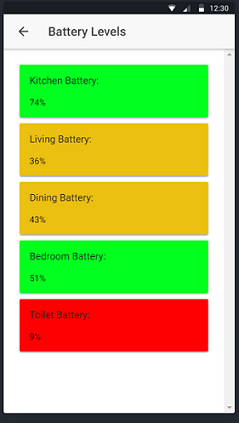
\includegraphics{battery}
\caption{A screenshot of the battery status page \label{bat}}
\end{wrapfigure}


~\\
This screen, in my application, has been designed to be able to be briefly glanced at, while still giving all the necessary information (battery levels). A user needs to be able to quickly view the screen without paying too much attention to it. The user does not care if a battery is at 90\% or 87\%, they simply care that a battery is at a low level and needs to be replaced or checked on. The app accomplishes this by colouring the battery levels.  This means that if a battery level is high, it will be coloured green, if the battery level is moderate, it will be coloured orange, and if the battery level is low it will be coloured red.

~\\
These colours play off fairly common colour significances. Green, orange, and yellow are commonly known as a "go" colour, a "moderate" colour, and a "warning" colour respectively. This colouring scheme allows a user to glance at the battery screen, and easily see if any sensors need to be checked or replaced.


~\\
\subsection{Battery Bar Graph - An Alternative}

An alternative battery screen design could have been a more graph focused alternative. This would have taken the form of a simple bar graph with each bar representing the level of battery at a specific sensor. The different bars could also be coloured by battery level like the actual battery screen. This could provide the advantage of the "glancibility" of the current design, along with the information that can be gained from a bar graph.



\subsection{Bar Graph}

The main part of the application is the home screen. This screen shows the current status of the sensors in the senior's house, the last known location, the time since the last recorded movement, and a graph of the areas where movement has been recorded. This last element is one of the most important as where motion has been detected recently is useful information. The visualisation of this information is an extremely important part of the app. This means that care had to be taken in choosing a method for the visualisation.

\begin{wrapfigure}{r}{0.4\textwidth}
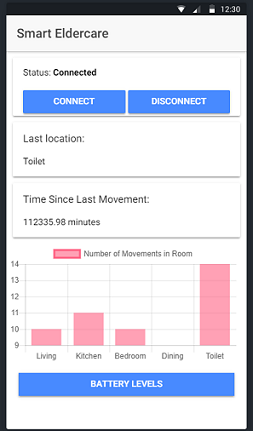
\includegraphics{home}
\caption{A screenshot of the home page, showing the bar graph \label{bat}}
\end{wrapfigure}


~\\
A bar graph was chosen to display this information, as it provided flexibility and worked well in a mobile app where space is limited and a larger, or different visualisation method may not have been suitable. The bar graph has a bar for each room in the house with a sensor, and the values increase each time movement is picked up on that sensor.


\subsection{Heat Map - An Alternative}

An alternative design for the home screen could have been a heat map. This would show each room in which a sensor is in, and be coloured based upon the frequency of movement in the room relative to the others. This would present some advantages, firstly, a map is useful, especially if a user is unfamiliar with the layout of the house. Secondly, it could be easy to glance at the map and see which areas have the most movement.

~\\
However, a heap map can present some major disadvantages, firstly, it would be difficult to fit a map of a large enough size to make sense in the limited space that is inherit in mobile design. Secondly, the house layout would be specific only to a single house, therefore the app could not be generic to multiple different houses with different layouts.

\section{Potential Issues}

\subsection{Battery and Fault Issues}

A major potential issue that this system could face would be the loss of a sensor in the house. If the senior is in the room that the lost sensor is in, the app could trigger a false alert when the senior is actually moving around. Additionally, it is possible that one or more sensors become faulty. This would present a major problem, as the app could not gather the data it would need to fulfil it's role. The app could then give false warnings when the senior is still moving around, or in the worst case, state a senior is moving around fine when in fact they are not moving and the app should be sending a warning.

~\\
A way to mitigate this issue would be to send a message to the user as soon as the application notes that a sensor is running very low on battery or is potentially faulty. Unfortunately, in the second case of the a sensor being potentially faulty, it can be difficult, if not impossible, to know if the sensor is faulty or not. In this case, if a sensor is suspected of being faulty, the user should still be notified of the sensor issues, and the user can deal with the problem from there.

\subsection{Other Movement Issues}

An additional major problem that this app could face is any other movement in the house that is not the senior. These other movements could result from pets, or from other people in the house. These movements could trigger the sensors and the app would think that the senior was moving when in fact it was another movement that the sensors were not meant to be tracking. A way to mitigate the pet issue is to place the sensors at a height at which the pets would not be able to trigger them, only the senior would be able to. Other people setting off the sensors would be a more difficult situation and one that seems fairly hard to mitigate. It would have to be assumed that if someone is moving in the house, that any potential issues with the senior can and will be handled.

\subsection{Senior Inactivity Issues}

Another problem that this app could face would be issues with senior inactivity. This would include the senior either sleeping or leaving the house. The sensors would then not pick up any movement and would send an alert when there is no need to send one. This could lead to false positives which would defeat the purpose of the app. A possible work around for this could be, when the senior is going to sleep, they push a button that times out the sensors for a period of time that they would sleep. A similar fix could be done for the senior leaving the house, when they leave they click a button, and the sensors are timed out, and when they get back the sensors are un-timed out.

\section{Reflection on IoT UX Design}

A major point that must be considered when designing user interfaces for IoT applications is that IoT systems generally have more points of failure than traditional systems. This means that more UX work has to be done around dealing with potential failures.

~\\
Additionally, the size constraints of the device on which the app is run must be considered. A mobile device will have a smaller screen which limits the application interface, especially in terms of visualisation techniques. This means, that for IoT mobile apps, it can be more difficult to create an effective mobile interface due to the constraints and nature of the devices and platform.

\end{document}